\section{Assassin's Creed: Revelations}

\begin{figure}[htbp]
\begin{center}
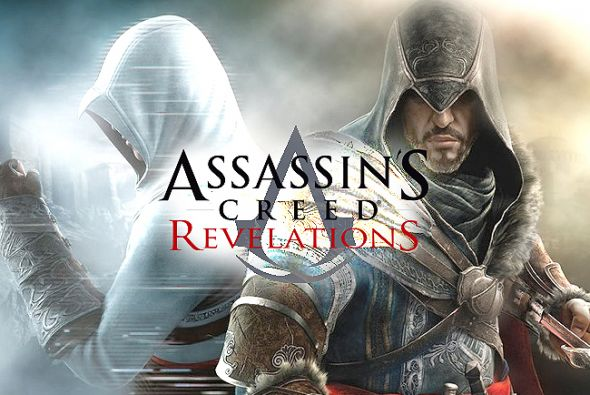
\includegraphics[width=.60\textwidth]{./imagenes/Revelations.jpg}
\caption{Assassin's Creed: Revelations}
\label{Assassin's Creed: Revelations}
\end{center}
\end{figure}
Assassin's Creed: Revelations\footnote{\url{http://assassinscreed.ubi.com/ac3/es-es/games/assassins-creed-revelations/index.aspx}} El juego comienza varios años después de Assassin's Creed: Brotherhood en el papel de Ezio, ya varios días con Lucy muerta, Desmond Miles en coma y Rebecca, Shaun y el misterioso William M. tratando de reanimar a Desmond, mediante el Animus. Desmond para tratar de salvarse, explorará los últimos días de las vidas de Altaïr Ibn-La'Ahad y Ezio Auditore, para crear un nexo de sincronización. 


\subsubsection{¿Por qué es uno de mis juegos favoritos?}
\begin{itemize}
\item[Luis Caviedes]Assassin’s Creed: Revelations hace gala a su nombre, ya que su historia une cabos sueltos de la franquicia y, sobre todo, sirve de nexo entre Ezio Auditore, Altaïr ibn La-Ahad y Desmond Miles, justamente los tres personajes jugables de este juego. La excelente jugabilidad es una marca de fábrica de la saga Assassin’s Creed. Revelations no es la excepción, otorgándonos un control de personaje soberbio. La ambientación de Constantinopla es sobrecogedora. Los detalles de los edificios, las mezquitas, los pueblos, el puerto, sorprenden gratamente. 
\end{itemize}